\documentclass[11pt]{article}
\usepackage[utf8]{inputenc}
\usepackage[T1]{fontenc}
\usepackage[francais]{babel}
\usepackage[francais]{layout}
\usepackage{tabularx,lipsum}
\selectlanguage{french}

\usepackage{array}
\newcolumntype{L}[1]{>{\raggedright\let\newline\\\arraybackslash\hspace{0pt}}m{#1}}
\newcolumntype{C}[1]{>{\centering\let\newline\\\arraybackslash\hspace{0pt}}m{#1}}
\newcolumntype{R}[1]{>{\raggedleft\let\newline\\\arraybackslash\hspace{0pt}}m{#1}}

% NE PAS CHANGER !!
\ifx \public \undefined \def\public{etudiants} \fi
\usepackage[\public]{tps}
\projettrue

% Titre du projet
\newcommand{\titreprojet}{Le dilemme du prisonnier}

\graphicspath{{imgs/}}

\begin{document}

\entete{\titreprojet}

\begin{introduction}
 Le sujet proposé, appelé <<le dilemme itéré des prisonniers>> doit aboutir à la réalisation d'un programme C destiné à simuler, de manière distribuée, l'évolution de populations en fonction de leur attitude face à un problème de tolérance.
\end{introduction}

\noindent
\textbf{Remarque :} Les deux premières sections représentent une exercice
de programmation générale. La troisième comporte un aspect système/réseau
et sera décisive pour l'évaluation. 

\bigskip

Le dilemme des prisonniers illustre la divergence entre l'intérêt personnel et l'intérêt collectif. 

En effet, le principe est le suivant, sachant que deux entités peuvent choisir entre coopérer ou trahir : 

\begin{itemize}
\item Si l'une trahit et l'autre coopère, celle qui trahit obtient un gain de T unités, et celle qui coopère obtient un gain (en général négatif) de D unités.

\item Lorsque les deux entités coopèrent, elles gagnent chacune C unités.

\item Lorsqu'elles trahissent toutes les deux, elles gagnent P unités pour s'être laissées piéger mutuellement. 
\end{itemize}

À défaut, les coefficients sont T = 5, D = 0, C = 3, P = 1. (cf. Figure~\ref{Coefs})

\begin{figure}[h]
 \centerline{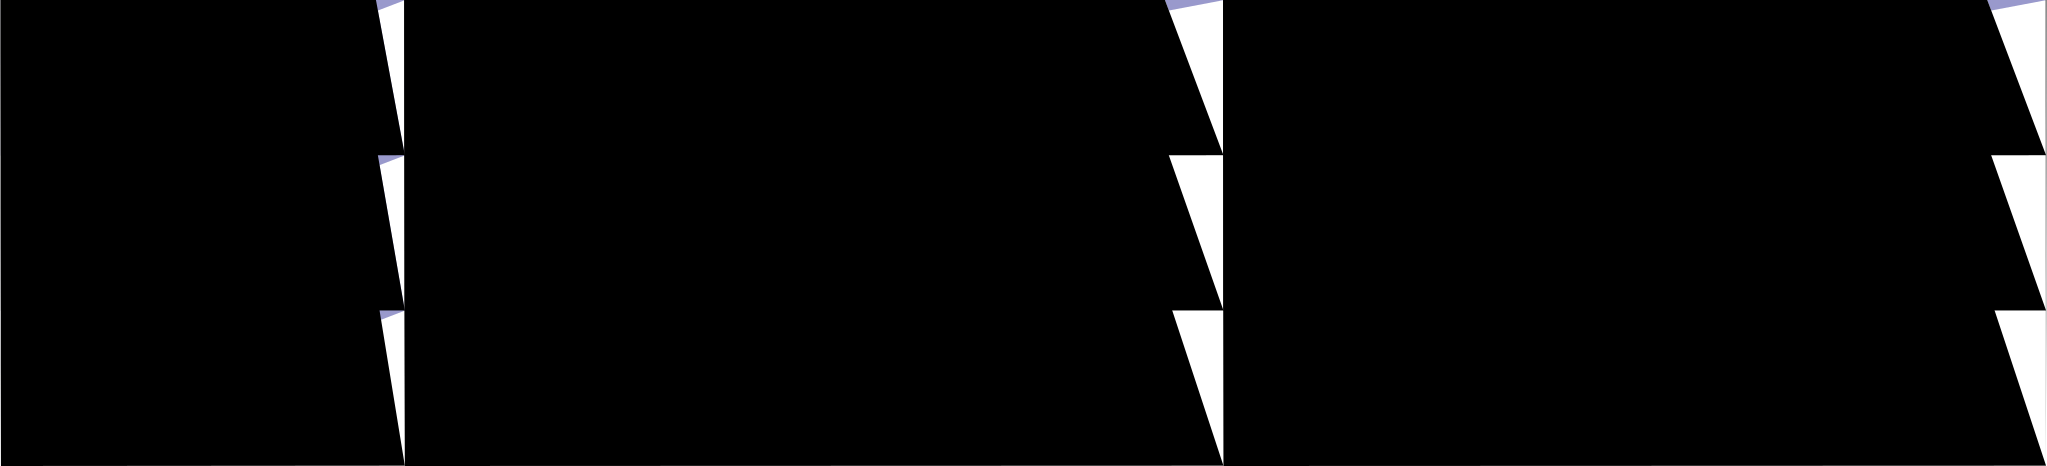
\includegraphics[width=10cm]{array.png}}
 \caption{Coefficients d'attribution des points}
 \label{Coefs}
\end{figure}

Lorsque la situation du dilemme des prisonniers est itérée, le jeu devient intéressant car il faut se demander quelle stratégie adopter face au comportement de l'entité adverse. Nous proposons d'étudier les onze stratégies suivantes : 

\begin{itemize}
    \item \textbf{GENTILLE :} Je coopère toujours 

    \item \textbf{MECHANTE :} Je trahis toujours

    \item \textbf{DONNANT-DONNANT :} Je coopère à la 1ère partie puis, je joue ce qu'a joué l'autre à la partie précédente

    \item \textbf{RANCUNIERE :} Je coopère mais dès que mon adversaire a trahi, je trahis toujours

    \item \textbf{PERIODIQUE-MECHANTE :} Je joue trahir, trahir, coopérer, trahir, trahir, coopérer…

    \item \textbf{PERIODIQUE-GENTILLE :} Je joue coopérer, coopérer, trahir, coopérer, coopérer, trahir…

    \item \textbf{MAJORITE-MOU :} Je joue ce que l'adversaire a joué en majorité, en cas d'égalité et à la première partie je coopère

    \item \textbf{MEFIANTE :} Je  trahis à la 1ère partie puis, je joue ce qu'a joué l'autre à la partie précédente

    \item \textbf{MAJORITE-DUR :} Je joue ce que l'adversaire a joué en majorité, en cas d'égalité et à la première partie je trahis

    \item \textbf{SONDEUR :} Aux trois premières parties, je joue trahir, coopérer, coopérer. Si aux parties 2 et 3 l'adversaire a coopéré, je trahis toujours, sinon j'opte pour la stratégie DONNANT-DONNANT 

    \item \textbf{DONNANT-DONNANT-DUR :} Je coopère sauf si mon adversaire trahit lors de l'une des 2 parties précédentes.
\end{itemize}

Note : Vous rendrez un rapport complet (exemples d'invocation des programmes, paramètres de compilation, etc) sur les différentes parties du projet ainsi que les sources des programmes demandés.
\textbf{Les sources devront compiler sans erreur sur les machines de la salle de TP C411}. 
À titre indicatif, le code d'une stratégie tient en au plus 4 lignes.

\section{Premiers essais}

Dans cette première partie nous testerons l'implémentation des stratégies présentées ci dessus.

\begin{itemize}
 \item Implémenter les 11 stratégies.
 \item Réaliser une fonction donnant le résultat de la confrontation de deux stratégies choisies à l'invocation du programme.
 \item Réaliser une fonction affichant le tableau des résultats des confrontations, lorsque les différentes stratégies combattent entre elles en un nombre fixé de coups.
 \item Réaliser une fonction cumulant le nombre de points que réalise une stratégie face à toutes les autres en un nombre de coup donné.
\end{itemize}

Vous rendrez pour cette partie un code source permettant d'afficher le tableau des confrontations et la table des cumuls de points pour un nombre de coups passé en paramètre. Exemple d'invocation : 

\begin{verbatim}
$ ./dileme1 1000
\end{verbatim}

Votre rapport contiendra un tableau du résultat des confrontations et un tableau du cumul de points pour 1000 coups joués.

\section{Simulation écologique}

Nous allons étudier l'évolution dynamique d'une population où chaque individu
obéit à une stratégie parmi les onze décrites ci-dessus. On va supposer que,
à la génération $n$, chaque individu confrontera chaque autre individu.
Dans la génération $n+1$, le taux de population d'une stratégie $s$ sera
proportionnel au nombre de points gagnés par les individus utilisant
cette stratégie, relativement aux points gagnés par tous les individus, 
à la génération $n$.

Formellement, soit $S$ l'ensemble des stratégies et $s,s'\in S$ ;
on note $g(s,s')$ le nombre
de points gagnés par un individu avec stratégie $s$ contre un individu avec
stratégie $s'$ lors d'une confrontation, et par $I^{n}_s$ le nombre d'individus utilisant
la stratégie $s$ à la génération $n$. Du coup,
$$P^n_s:=I^n_s\cdot\bigg(g(s,s)\cdot(I^n_s-1)+\sum_{s'\ne s}g(s,s')\cdot I^n_{s'}\bigg)$$
est le nombre de points gagnés par les individus de stratégie $s$ à la génération $n$, et à la génération suivante, tant que $I^{n}_s>0$ :
$$I^{n+1}_s:=e_{n+1}\cdot {P^n_s\over \sum_{s'\in S} P^n_{s'}},$$
et $I^{n+1}_s=0$ sinon
où $e_{n+1}$ est la taille de la population à la génération $n+1$.

%Une simulation écologique représente l'évolution de populations appliquant différentes stratégies.

%Chaque stratégie dispose d'une population de $x$ entités.
%$a(n)=x$ est l'effectif de la stratégie A à la génération $n$.
%Chaque entité affronte toutes les autres entités de sa stratégie, sauf elle même, et des autres.
%Les points marqués par la stratégie A à la génération $n$ sont notés $g(A,n)$.
%$t(n)$ est le total des points gagnés par toutes les stratégies.

%À effectif $e$ constant, nous avons $e=a(n)+b(n)+...=a(n+1)+b(n+1)+...$.

%L'évolution de la population d'une stratégie est $a(n+1) = e.\frac{a(n).g(A,n)}{t(n)}$

\medskip

Votre tâche est la suivante :
\begin{itemize}
 \item Écrire un code réalisant une simulation écologique.
  Au départ, chaque stratégie possède le même nombre d'individus, et la
  taille de la population restera constante.
\end{itemize}

Vous rendrez un code générant un tableau de résultat pour un nombre de génération et un effectif passé en argument.
Exemple d'invocation pour 30 générations et une population de départ de 100 entités par stratégie :

\begin{verbatim}
$ ./dileme2 30 100
\end{verbatim}

Votre rapport contiendra un graphique représentant l'évolution d'une population de 100 entités sur 30 générations.

\section{Simulation distribuée}

Nous allons maintenant étudier l'évolution simultanée de la population dans
plusieurs villes. Une ville se distingue des autres par les paramètres
suivants :

\begin{itemize}
\item la taille de sa population ;
\item le sous-ensemble des stratégies permises dans ses murs ;
\item la valeur des paramètres $D,C,P,T$.
\end{itemize}

Par ailleurs, un habitant peut décider, avec une certaine
probabilité, de migrer dans une autre ville. Chaque ville
sera simulée sur une autre machine et communiquera l'état
de sa population à une machine centrale.

\medskip

Votre tâche est d'écrire un code permettant de :
\begin{itemize}
\item simuler une ville ;
\item lancer simultanément la simulation de plusieurs villes avec leurs paramètres
   sur des machines distantes ;
\item observer l'évolution de toutes les villes sur votre ordinateur.
\end{itemize}

Chaque ville doit donc communiquer périodiquement l'état de sa population
(sa composition, sa taille, le nombre de points gagnés)
à une machine centrale, et les villes doivent communiquer entre elles pour
permettre aux individus de migrer.

Le rapport, rédigé soigneusement, décrira tous les choix que vous aurez effectué ainsi que l'invocation du programme et toutes les modalités de mise en œuvre.
Des exemples d'invocations et de résultats obtenus illustreront votre travail.

\subsubsection*{Variations possibles}

Certains détails de la simulation sont laissés à votre imagination.
Par exemple, on peut laisser la taille de la population évoluer en
fonction de la prospérité d'une ville, permettre aux individus de
muter vers une autre stratégie, limiter la migration à un ensemble
de villes <<voisines>>\ldots En tout cas, documentez vos choix.

\end{document}
